\hypertarget{Partial_8h}{
\section{Partial.h File Reference}
\label{Partial_8h}\index{Partial.h@{Partial.h}}
}
{\tt \#include \char`\"{}Xml\-Reader.h\char`\"{}}\par
{\tt \#include $<$fstream$>$}\par
{\tt \#include $<$iostream$>$}\par
{\tt \#include $<$list$>$}\par
{\tt \#include \char`\"{}Types.h\char`\"{}}\par
{\tt \#include \char`\"{}Parameter\-Lib.h\char`\"{}}\par
{\tt \#include \char`\"{}Track.h\char`\"{}}\par
{\tt \#include \char`\"{}Reverb.h\char`\"{}}\par


Include dependency graph for Partial.h:\begin{figure}[H]
\begin{center}
\leavevmode
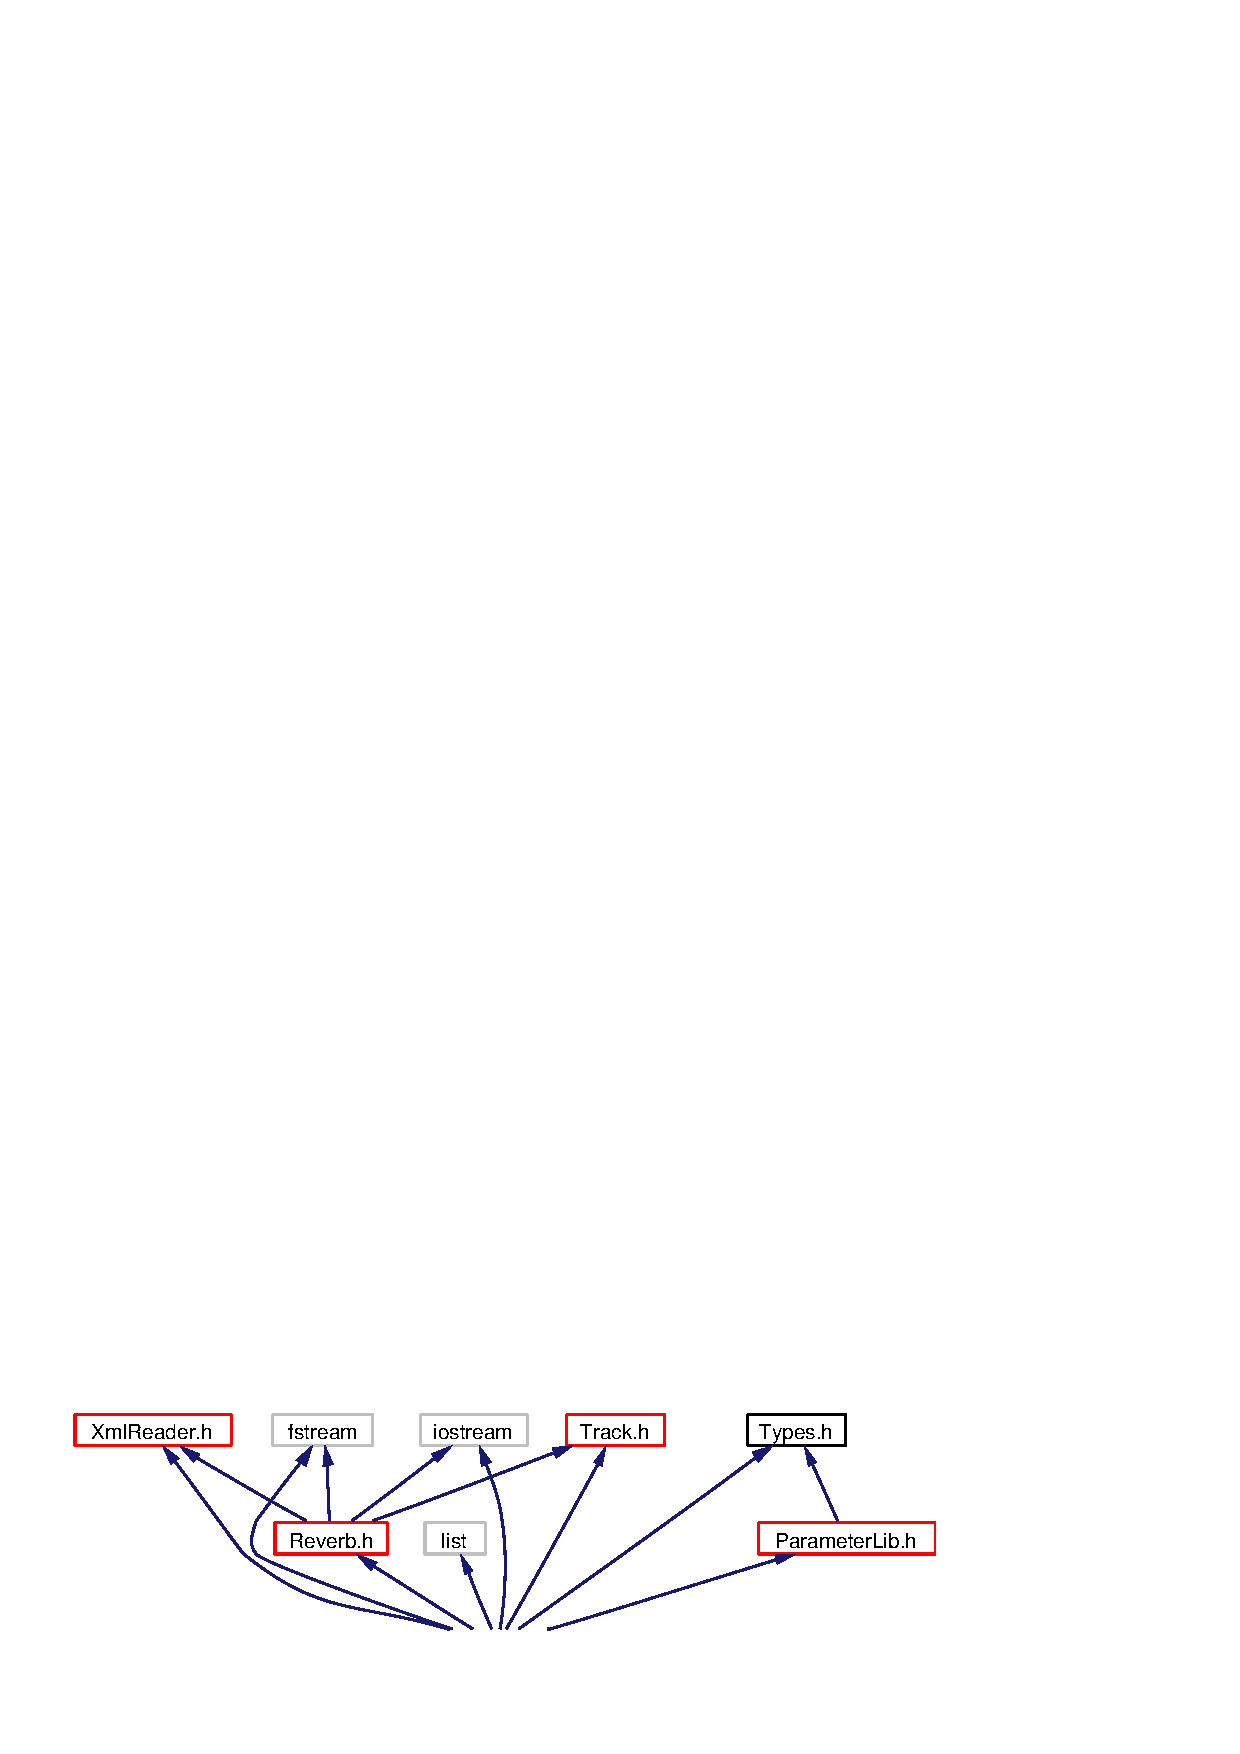
\includegraphics[width=224pt]{Partial_8h__incl}
\end{center}
\end{figure}


This graph shows which files directly or indirectly include this file:\begin{figure}[H]
\begin{center}
\leavevmode
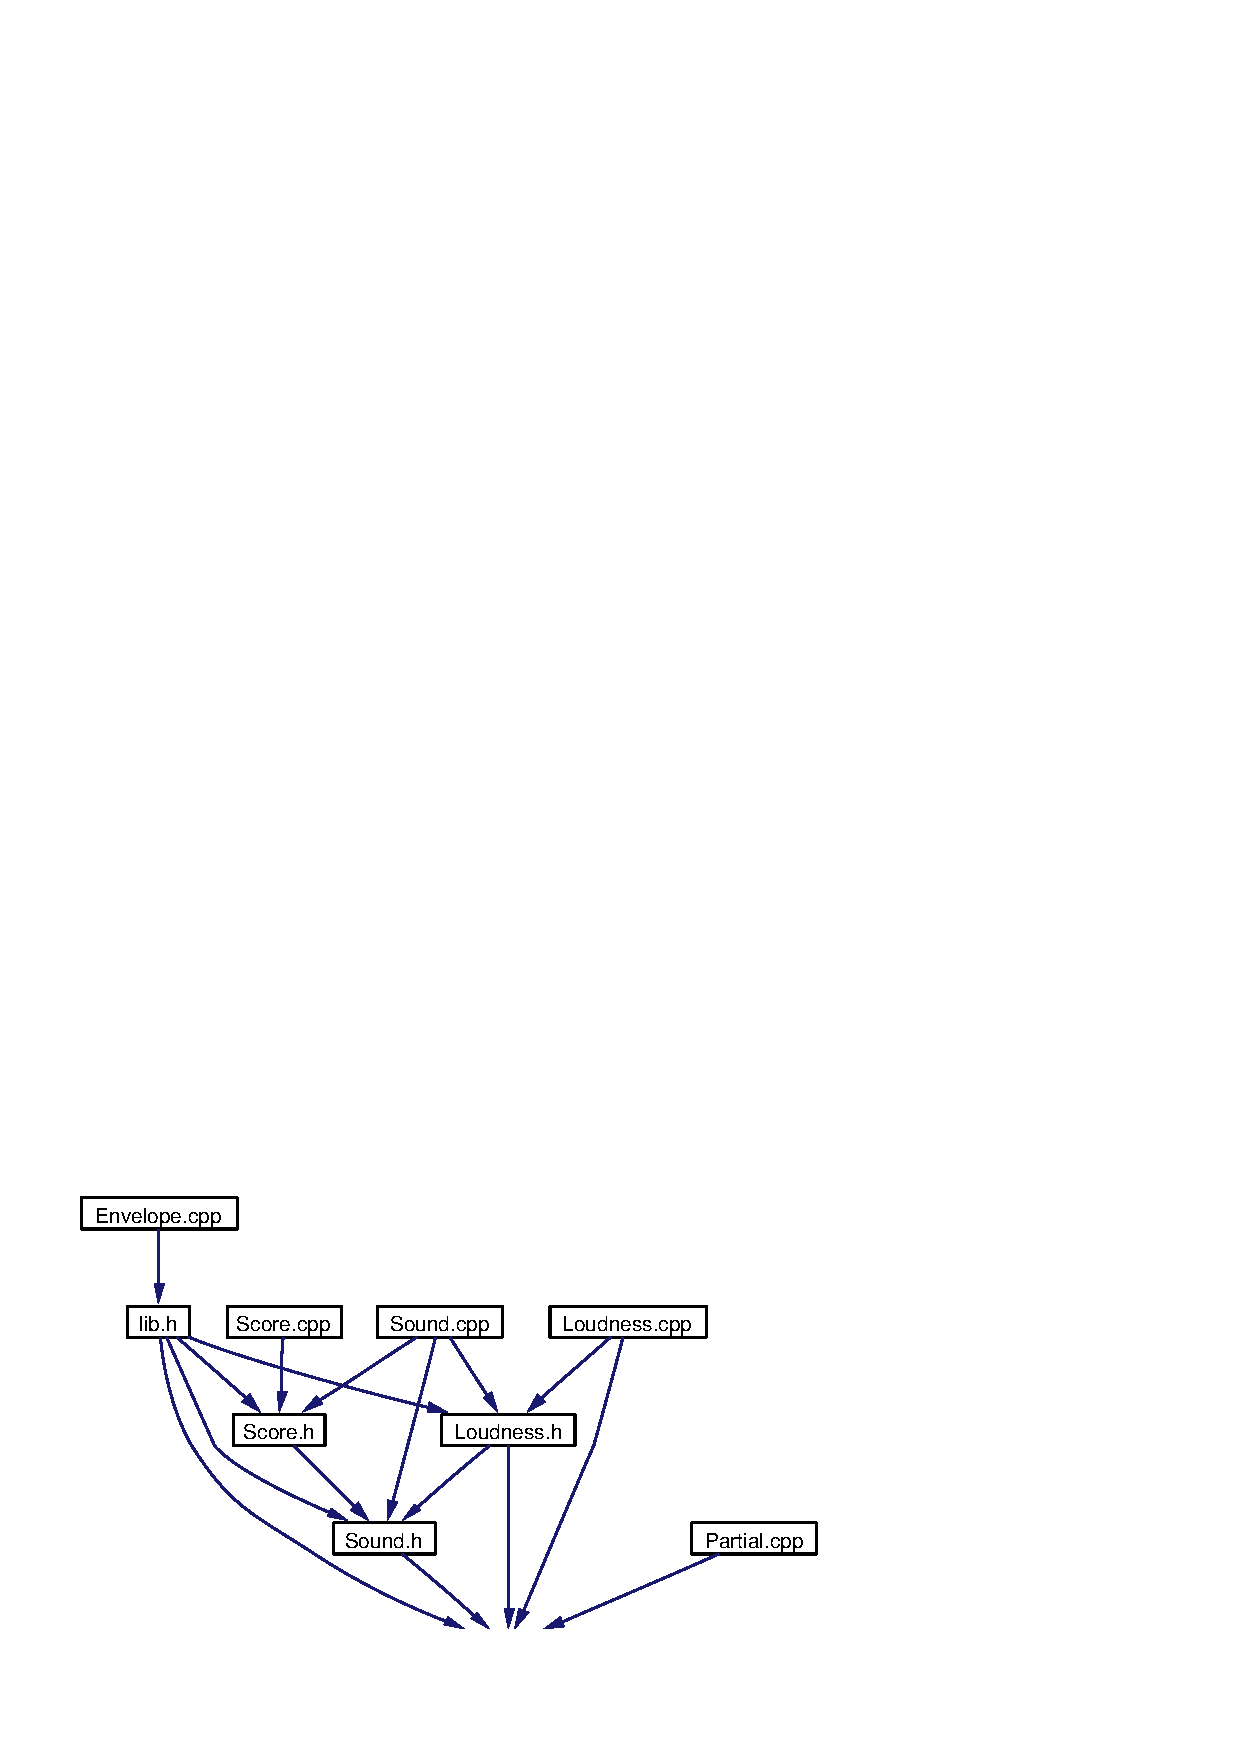
\includegraphics[width=196pt]{Partial_8h__dep__incl}
\end{center}
\end{figure}
\subsection*{Classes}
\begin{CompactItemize}
\item 
class \hyperlink{classPartial}{Partial}
\end{CompactItemize}
\subsection*{Enumerations}
\begin{CompactItemize}
\item 
enum \hyperlink{Partial_8h_a19}{Partial\-Static\-Param} \{ \par
\hyperlink{Partial_8h_a19a0}{RELATIVE\_\-AMPLITUDE}, 
\par
\hyperlink{Partial_8h_a19a1}{PARTIAL\_\-NUM}, 
\par
\hyperlink{Partial_8h_a19a2}{WAVE\_\-TYPE}
 \}
\item 
enum \hyperlink{Partial_8h_a20}{Partial\-Dynamic\-Param} \{ \par
\hyperlink{Partial_8h_a20a3}{FREQUENCY}, 
\par
\hyperlink{Partial_8h_a20a4}{WAVE\_\-SHAPE}, 
\par
\hyperlink{Partial_8h_a20a5}{TREMOLO\_\-AMP}, 
\par
\hyperlink{Partial_8h_a20a6}{TREMOLO\_\-RATE}, 
\par
\hyperlink{Partial_8h_a20a7}{VIBRATO\_\-AMP}, 
\par
\hyperlink{Partial_8h_a20a8}{VIBRATO\_\-RATE}, 
\par
\hyperlink{Partial_8h_a20a9}{PHASE}, 
\par
\hyperlink{Partial_8h_a20a10}{LOUDNESS\_\-SCALAR}, 
\par
\hyperlink{Partial_8h_a20a11}{FREQ\_\-ENV}, 
\par
\hyperlink{Partial_8h_a20a12}{DETUNING\_\-ENV}, 
\par
\hyperlink{Partial_8h_a20a13}{AMPTRANS\_\-AMP\_\-ENV}, 
\par
\hyperlink{Partial_8h_a20a14}{AMPTRANS\_\-RATE\_\-ENV}, 
\par
\hyperlink{Partial_8h_a20a15}{FREQTRANS\_\-AMP\_\-ENV}, 
\par
\hyperlink{Partial_8h_a20a16}{FREQTRANS\_\-RATE\_\-ENV}, 
\par
\hyperlink{Partial_8h_a20a17}{AMPTRANS\_\-WIDTH}, 
\par
\hyperlink{Partial_8h_a20a18}{FREQTRANS\_\-WIDTH}
 \}
\end{CompactItemize}


\subsection{Detailed Description}
Defines a \hyperlink{classPartial}{Partial} object, as well as the static and dynamic parameters that pertain to said object.

Definition in file \hyperlink{Partial_8h-source}{Partial.h}.

\subsection{Enumeration Type Documentation}
\hypertarget{Partial_8h_a20}{
\index{Partial.h@{Partial.h}!PartialDynamicParam@{PartialDynamicParam}}
\index{PartialDynamicParam@{PartialDynamicParam}!Partial.h@{Partial.h}}
\subsubsection[PartialDynamicParam]{\setlength{\rightskip}{0pt plus 5cm}enum \hyperlink{Partial_8h_a20}{Partial\-Dynamic\-Param}}}
\label{Partial_8h_a20}


Defines the Dynamic parameters that can be set for a \hyperlink{classPartial}{Partial} object.\begin{itemize}
\item FREQUENCY\begin{itemize}
\item The pitch at which a partial is heard.\item Set in Hz. (no bounds checking)\end{itemize}
\item WAVE\_\-SHAPE\begin{itemize}
\item How the partial changes it's amplitude over time.\item \hyperlink{classEnvelope}{Envelope} should start and end at y=0; otherwise \char`\"{}clicks\char`\"{} and \char`\"{}pops\char`\"{} will be created\end{itemize}
\item TREMOLO\_\-AMP\begin{itemize}
\item The amplitude of tremolo (size of the effect).\item Given as a scaling factor to amplitude.\end{itemize}
\item TREMOLO\_\-RATE\begin{itemize}
\item Given in Hz. (see vibrato rate)\end{itemize}
\item VIBRATO\_\-AMP\begin{itemize}
\item The amplitude of vibrato (size of the effect).\item Given as a scaling factor to frequency.\end{itemize}
\item VIBRATO\_\-RATE\begin{itemize}
\item Given in Hz. (6 Hz is a \char`\"{}normal\char`\"{} vibrato)\end{itemize}
\item FREQUENCY\_\-DEVIATION $\ast$$\ast$$\ast$$\ast$Commmented out (i.e. not used anywhere, but can be put back in)$\ast$$\ast$$\ast$$\ast$$\ast$\begin{itemize}
\item Specifies how randomly scaled the frequencies of this partial will be.\item Range \mbox{[}0 - 1\mbox{]}\item Could be specified as a value or as an envelope which will affect the frequency. Exactly the same effect can be obtained by using GLISSANDO\_\-ENV or DETUNING\_\-ENV. See comment for glissando envelope.\end{itemize}
\item LOUDNESS\_\-SCALAR\begin{itemize}
\item Not to be set by users.\item This variable is set by the \hyperlink{classLoudness}{Loudness} routines.\item The scaling factor is then taken into account at every sample.\end{itemize}
\item GLISSANDO\_\-ENV $\ast$$\ast$$\ast$$\ast$$\ast$$\ast$$\ast$Commented Out (i.e. not used anywhere, but can be put back in) $\ast$$\ast$$\ast$$\ast$$\ast$\begin{itemize}
\item This is a glissando envelope. It is multiplied by the\item frequency at every point. Thus, if you leave it at 1.0 (The default, it will not affect anything). If you leave it at 1.0 for most of the sound, then interpolate it down to 0.5, the partial will trail off (by an octave down) at the end of the sound.\item The y values for this envelope can be any positive number. a value of 0 will kill the sound (0 frequency), and too high of a value could make the frequency inaudible or above Nyquist (no bounds checking).\end{itemize}
\item DETUNING\_\-ENV $\ast$$\ast$$\ast$$\ast$$\ast$$\ast$$\ast$$\ast$ (Commmented Out) $\ast$$\ast$$\ast$$\ast$$\ast$$\ast$$\ast$$\ast$$\ast$\begin{itemize}
\item used to gradually tune or detune a partial. It's an envelope, and acts just like a glissando envelope, but more general.\end{itemize}
\item AMPTRANS\_\-AMP\_\-ENV\begin{itemize}
\item used to control the value of amplitude transients\item the value of the amp envelope is a maximum transient modifier\item this value is multiplied by a random percentage and then used to modify the amplitude as follows: If the value after the percentage is applied is 0.7, then the amplitude will be 1.7 or 0.3 times its original value.\end{itemize}
\item AMPTRANS\_\-RATE\_\-ENV\begin{itemize}
\item used to control the rate of amplitude transients\item the value of the rate envelope is the percentage chance of a transient occuring at that particular time\end{itemize}
\item FREQTRANS\_\-AMP\_\-ENV\begin{itemize}
\item used to control the amplitude of frequency transients\item see AMPTRANS\_\-AMP\_\-ENV for an explanation\end{itemize}
\item FREQTRANS\_\-RATE\_\-ENV\begin{itemize}
\item used to control the rate of frequency transients\item see AMPTRANS\_\-RATE\_\-ENV for an explanation\end{itemize}
\item AMPTRANS\_\-WIDTH\begin{itemize}
\item the width of any amplitude transient in samples\item defaults to 1103, or 0.025 seconds.\end{itemize}
\item FREQTRANS\_\-WIDTH -the width of any frequency transient in samples\begin{itemize}
\item defaults to 1103, or 0.025 seconds. \end{itemize}
\end{itemize}
\begin{Desc}
\item[Enumeration values: ]\par
\begin{description}
\index{FREQUENCY@{FREQUENCY}!Partial.h@{Partial.h}}\index{Partial.h@{Partial.h}!FREQUENCY@{FREQUENCY}}\item[{\em 
\hypertarget{Partial_8h_a20a3}{
FREQUENCY}
\label{Partial_8h_a20a3}
}]\index{WAVE_SHAPE@{WAVE\_\-SHAPE}!Partial.h@{Partial.h}}\index{Partial.h@{Partial.h}!WAVE_SHAPE@{WAVE\_\-SHAPE}}\item[{\em 
\hypertarget{Partial_8h_a20a4}{
WAVE\_\-SHAPE}
\label{Partial_8h_a20a4}
}]\index{TREMOLO_AMP@{TREMOLO\_\-AMP}!Partial.h@{Partial.h}}\index{Partial.h@{Partial.h}!TREMOLO_AMP@{TREMOLO\_\-AMP}}\item[{\em 
\hypertarget{Partial_8h_a20a5}{
TREMOLO\_\-AMP}
\label{Partial_8h_a20a5}
}]\index{TREMOLO_RATE@{TREMOLO\_\-RATE}!Partial.h@{Partial.h}}\index{Partial.h@{Partial.h}!TREMOLO_RATE@{TREMOLO\_\-RATE}}\item[{\em 
\hypertarget{Partial_8h_a20a6}{
TREMOLO\_\-RATE}
\label{Partial_8h_a20a6}
}]\index{VIBRATO_AMP@{VIBRATO\_\-AMP}!Partial.h@{Partial.h}}\index{Partial.h@{Partial.h}!VIBRATO_AMP@{VIBRATO\_\-AMP}}\item[{\em 
\hypertarget{Partial_8h_a20a7}{
VIBRATO\_\-AMP}
\label{Partial_8h_a20a7}
}]\index{VIBRATO_RATE@{VIBRATO\_\-RATE}!Partial.h@{Partial.h}}\index{Partial.h@{Partial.h}!VIBRATO_RATE@{VIBRATO\_\-RATE}}\item[{\em 
\hypertarget{Partial_8h_a20a8}{
VIBRATO\_\-RATE}
\label{Partial_8h_a20a8}
}]\index{PHASE@{PHASE}!Partial.h@{Partial.h}}\index{Partial.h@{Partial.h}!PHASE@{PHASE}}\item[{\em 
\hypertarget{Partial_8h_a20a9}{
PHASE}
\label{Partial_8h_a20a9}
}]\index{LOUDNESS_SCALAR@{LOUDNESS\_\-SCALAR}!Partial.h@{Partial.h}}\index{Partial.h@{Partial.h}!LOUDNESS_SCALAR@{LOUDNESS\_\-SCALAR}}\item[{\em 
\hypertarget{Partial_8h_a20a10}{
LOUDNESS\_\-SCALAR}
\label{Partial_8h_a20a10}
}]\index{FREQ_ENV@{FREQ\_\-ENV}!Partial.h@{Partial.h}}\index{Partial.h@{Partial.h}!FREQ_ENV@{FREQ\_\-ENV}}\item[{\em 
\hypertarget{Partial_8h_a20a11}{
FREQ\_\-ENV}
\label{Partial_8h_a20a11}
}]\index{DETUNING_ENV@{DETUNING\_\-ENV}!Partial.h@{Partial.h}}\index{Partial.h@{Partial.h}!DETUNING_ENV@{DETUNING\_\-ENV}}\item[{\em 
\hypertarget{Partial_8h_a20a12}{
DETUNING\_\-ENV}
\label{Partial_8h_a20a12}
}]\index{AMPTRANS_AMP_ENV@{AMPTRANS\_\-AMP\_\-ENV}!Partial.h@{Partial.h}}\index{Partial.h@{Partial.h}!AMPTRANS_AMP_ENV@{AMPTRANS\_\-AMP\_\-ENV}}\item[{\em 
\hypertarget{Partial_8h_a20a13}{
AMPTRANS\_\-AMP\_\-ENV}
\label{Partial_8h_a20a13}
}]\index{AMPTRANS_RATE_ENV@{AMPTRANS\_\-RATE\_\-ENV}!Partial.h@{Partial.h}}\index{Partial.h@{Partial.h}!AMPTRANS_RATE_ENV@{AMPTRANS\_\-RATE\_\-ENV}}\item[{\em 
\hypertarget{Partial_8h_a20a14}{
AMPTRANS\_\-RATE\_\-ENV}
\label{Partial_8h_a20a14}
}]\index{FREQTRANS_AMP_ENV@{FREQTRANS\_\-AMP\_\-ENV}!Partial.h@{Partial.h}}\index{Partial.h@{Partial.h}!FREQTRANS_AMP_ENV@{FREQTRANS\_\-AMP\_\-ENV}}\item[{\em 
\hypertarget{Partial_8h_a20a15}{
FREQTRANS\_\-AMP\_\-ENV}
\label{Partial_8h_a20a15}
}]\index{FREQTRANS_RATE_ENV@{FREQTRANS\_\-RATE\_\-ENV}!Partial.h@{Partial.h}}\index{Partial.h@{Partial.h}!FREQTRANS_RATE_ENV@{FREQTRANS\_\-RATE\_\-ENV}}\item[{\em 
\hypertarget{Partial_8h_a20a16}{
FREQTRANS\_\-RATE\_\-ENV}
\label{Partial_8h_a20a16}
}]\index{AMPTRANS_WIDTH@{AMPTRANS\_\-WIDTH}!Partial.h@{Partial.h}}\index{Partial.h@{Partial.h}!AMPTRANS_WIDTH@{AMPTRANS\_\-WIDTH}}\item[{\em 
\hypertarget{Partial_8h_a20a17}{
AMPTRANS\_\-WIDTH}
\label{Partial_8h_a20a17}
}]\index{FREQTRANS_WIDTH@{FREQTRANS\_\-WIDTH}!Partial.h@{Partial.h}}\index{Partial.h@{Partial.h}!FREQTRANS_WIDTH@{FREQTRANS\_\-WIDTH}}\item[{\em 
\hypertarget{Partial_8h_a20a18}{
FREQTRANS\_\-WIDTH}
\label{Partial_8h_a20a18}
}]\end{description}
\end{Desc}



Definition at line 134 of file Partial.h.\hypertarget{Partial_8h_a19}{
\index{Partial.h@{Partial.h}!PartialStaticParam@{PartialStaticParam}}
\index{PartialStaticParam@{PartialStaticParam}!Partial.h@{Partial.h}}
\subsubsection[PartialStaticParam]{\setlength{\rightskip}{0pt plus 5cm}enum \hyperlink{Partial_8h_a19}{Partial\-Static\-Param}}}
\label{Partial_8h_a19}


Defines the static parameters that can be set for a \hyperlink{classPartial}{Partial} object.\begin{itemize}
\item RELATIVE\_\-AMPLITUDE\begin{itemize}
\item Used by \hyperlink{classLoudness}{Loudness} to balance the amplitude of partials.\item Set these values in any range you like.\end{itemize}
\item PARTIAL\_\-NUM\begin{itemize}
\item Defines the number partial.\item 0 is the lowest partial.\item Currently only used for Frequency Deviation calculations.\end{itemize}
\item WAVE\_\-TYPE\begin{itemize}
\item Specify type of wave \end{itemize}
\end{itemize}
\begin{Desc}
\item[Enumeration values: ]\par
\begin{description}
\index{RELATIVE_AMPLITUDE@{RELATIVE\_\-AMPLITUDE}!Partial.h@{Partial.h}}\index{Partial.h@{Partial.h}!RELATIVE_AMPLITUDE@{RELATIVE\_\-AMPLITUDE}}\item[{\em 
\hypertarget{Partial_8h_a19a0}{
RELATIVE\_\-AMPLITUDE}
\label{Partial_8h_a19a0}
}]\index{PARTIAL_NUM@{PARTIAL\_\-NUM}!Partial.h@{Partial.h}}\index{Partial.h@{Partial.h}!PARTIAL_NUM@{PARTIAL\_\-NUM}}\item[{\em 
\hypertarget{Partial_8h_a19a1}{
PARTIAL\_\-NUM}
\label{Partial_8h_a19a1}
}]\index{WAVE_TYPE@{WAVE\_\-TYPE}!Partial.h@{Partial.h}}\index{Partial.h@{Partial.h}!WAVE_TYPE@{WAVE\_\-TYPE}}\item[{\em 
\hypertarget{Partial_8h_a19a2}{
WAVE\_\-TYPE}
\label{Partial_8h_a19a2}
}]\end{description}
\end{Desc}



Definition at line 58 of file Partial.h.